
We investigate and discuss our results for the Biological Process (BP) category in the main text. We include the results for the evaluation of Molecular Function (MF) in the supplementary material. \murali{Rather than simply put the MF results in the supplement, we will have to refer to them in meaningful ways in the main text.}

We evaluated each method using leave-one-species-out (LOSO) validation with 19 bacterial species where we mimicked the challenge of making large-scale functional predictions for the genome of a newly-sequenced species %where none of the genes have any previous annotations. 
that has no previous annotations.
We constructed a multi-species network, left out the annotations of all genes for each species in turn, and used the annotations of the other 18 organisms to make predictions for the left-out species (see \cref{fig:leave-one-species-out}). 
First, we tested the trade-off between accuracy and speed for \sinksource by varying either $\alpha$ or the number of iterations, \murali{We have to describe the other sections as well.}
and later use the selected parameters as we scale-up to 200 bacterial species.
%We then evaluated three network propagation methods---\sinksource, \genemania and \birgrank---against the baseline \localplus method.
%Then we analyze the compare the effect of choosing different BLAST \eval cutoffs and STRING cutoffs to build the multi-species network


\subsection{Trade-off between Accuracy and Speed}
\label{sec:tradeoff-accuracy-speed}

%\murali{State the goals of the experiment (We first ...), then the way you performed the experiment, then refer to the figure and describe, the results.}
By design, \sinksource converges faster, i.e., with a smaller number of iterations as we decrease the parameter $\alpha$  \murali{Refer to lemma in the supplement.} Additionally, for a fixed $\alpha$, \sinksource terminates faster as we decrease the number of iterations. Therefore, we sought to test the trade-off between accuracy and speed by varying either $\alpha$ or the number of iterations before we stopped \sinksource. 
%\murali{Where have you defined ``stopping criteria'' before? I modified the sentence since it was potentially confusing as written. It could mean that $\alpha$ controls accuracy and the other criterion controls speed. But that is not what you intended to say, is it?}


First, we ran \sinksource for eight different values of $\alpha$, namely, 1, 0.99, 0.95, 0.9, 0.8, 0.7, 0.6, and 0.5. 
%\murali{You are in the middle of describing the setup for these experiments. Don't mention results here. Mention them in the next para. "which is double the number of iterations required to fix the rankings for $\alpha = 0.9$, and which resulted in an average $\epsilon$ of \e{-4}" \jeff{need to show this data in the supp.}.} 
% no longer five-fold cross-validation
For each value, we performed the \loso evaluation for each of the 19 bacterial species using the \SSN (\eval $\leq 0.1$) integrated with STRING and only annotations with experimental evidence codes. We considered 319 biological process GO terms, each with at least 50 annotations summed over all 19 organisms. For each "left-out" species, we limited the evaluation to the GO terms with at least 10 annotations in that species.
For values of $\alpha < 1$, we executed \sinksource to convergence, i.e., we used as many iterations as needed to fix the relative rankings of the positive and negative examples in the left-out species, ignoring the bounds for the other examples in our test for fixed ordering.
%executed \sinksource to convergence, i.e., until every left-out positive or negative node had a distinct upper and lower bound. We called the resulting ranking of nodes as the "fixed ordering." \murali{What do we do about ties? Where do we discuss this issue?} \jeff{If they're fixed compared to all other nodes, we fix their ranking as well. I made a note of this in the methods.}
For $\alpha = 1.0$, the upper bound on the node score we can prove is trivially equal to unity in each iteration. 
%\murali{"Squeeze upper bound": This phrase does not sound good. You have to refer to a lemma or a theorem or "our upper bound". I also don't want Squeeze to appear in the paper anywhere but the place where we prove our theory.} 
Therefore, we stopped \sinksource after 1000 iterations. 

We explored the effect of varying $\alpha$ on the accuracy of \sinksource by comparing the resulting distributions of \fmax values (\cref{fig:sinksource-speed-vs-accuracy}a). 
The median \fmax value did decrease gradually as we decreased $\alpha$. 
For $\alpha \leq 0.8$, we observed a statistically significant difference compared to $\alpha = 1.0$ (uncorrected \pval $\leq$ 0.1).
However, we did not observe a significant difference between the distributions for $\alpha = 1.0$, and $\alpha = 0.99$, $\alpha = 0.95$, and $\alpha = 0.9$, with the median of differences between the \fmax for each GO term of 0.0, 0.002, and 0.005 respectively (rank-sum test, uncorrected \pval 0.45, 0.28, and 0.17 respectively).
%However, we did not observe a statistically-significant difference between the distributions for $\alpha = 1.0$ and $\alpha = 0.8$ (rank-sum test, uncorrected \pval = 0.08).
%We note that the rank-sum test could lead to overly-optimistic \pval{}s as GO terms are not fully independent from each other.  \murali{Use brackets only for small phrases and not for multiple sentences. More importantly, why mention over optimism here when the \pval{}s are not significant? Over-optimism is an issue only if the p-values are small.}
%We recognize the choice of $\alpha$ for \sinksource is somewhat arbitrary and depends on specific use cases. In our experiments, for $\alpha < 0.8$, the rank-sum \pval fell below 0.05, 
We chose $\alpha = 0.95$ for subsequent analyses.  

% # of iterations
Next, we considered varying the number of iterations for which we ran \sinksource. We first executed \sinksource to convergence, i.e., the node orderings were fixed.
We then re-executed \sinksource and for each $i > 0$, we compared how similar the node ranking after iteration $i$ was to the fixed ordering using \ktau, a measure of rank correlation. Given two different rankings of the nodes, this measure counts the fraction of node pairs that are not inverted, i.e., the fraction of node pairs $u$ and $v$ such that $u$ appears before $v$ in both rankings or vice-versa. Thus, the closer $\tau$ is to unity, the more similar are the two rankings. For each GO term, we recorded the number of iterations needed to reach a correlation of 0.9, 0.95, 0.99, and 1.0 (\cref{fig:sinksource-speed-vs-accuracy}b). 
%, and the largest stretch of nodes with overlapping upper or lower bounds. 
%The \ktau statistic will advise us as to how many iterations are needed to approximate the fixed ranking.
The median number of iterations required to fix the node ordering was 359. Interestingly, we observed that \sinksource computed this ranking sooner with a median of 170 iterations (see \cref{fig:sinksource-speed-vs-accuracy}b, \ktau = 1.0); subsequent iterations did not change the ordering but were necessary to guarantee that it would not be modified by more iterations. 
% precision problem:
% This is partially due to the limited 80-bit precision of numpy.  At about 200 iterations, the maximum precision for node scores is reached, and the maximum difference of node scores from one iteration to the next drops to 0 meaning the node scores cannot be approximated any better. Squeeze maintains a single value $x$ to compute the upper bound for all nodes which is the lower bound plus $x$. The upper bound value $x$ does not require many digits to compute, and can be stored with leading zeros meaning it does not suffer from loss of precision allowing us to better approximate it the upper bounds. After 400 iterations, the upper-bound is small enough to ensure the nodes have distinct upper and lower bounds. As we are primarily concerned with the values of the first few digits and not the full precision, we decided not to bother computing the full precision on a platform such as matlab 
Even more strikingly, after a median of 29 and 18 iterations, \ktau was already as high as 0.95 and 0.90, respectively.
These results suggested that while about 360 iterations may be required to provably fix the rankings of the left-out positive and negative nodes, reducing the number of iterations by a factor of 20 does not have a material impact of the relative orderings of most of the positive and negative node pairs. Moreover, fewer iterations may not be deleterious to the accuracy of \sinksource during evaluation.

To test this hypothesis, we fixed $\alpha = 0.95$, ran \sinksource for eight different number of iterations (400, 200, 50, 20, 10, 5, 2, and 1, and recorded the
% node rankings \murali{Where are the results for node ranking?} 
%\jeff{For 10 iterations, the median \ktau is about 0.85, 5 is 0.79, 3 is 0.7 and 1 is 0.17} and 
\fmax values after \loso validation (\cref{fig:sinksource-speed-vs-accuracy}c). The \fmax distribution for 400 iterations was statistically indistinguishable from the distribution for each of the next four largest number of iterations (200, 50, 20, and 10, rank-sum test, \pval $\geq 0.25$).
%, with medians of \fmax differences equal to 0 for $\geq 20$ iterations, and 0.004 comparing 400 to 10 iterations.
We concluded that decreasing the number of iterations by as large a factor as 40 did not affect the overall distribution of \loso performance. 
% running time
%The running time improved by a factor of 50 (331 minutes for \sinksource with $\alpha = 1.0$ for 1000 iterations vs. 6.6 minutes for 20 iterations with $\alpha = 0.8$, \fig \ref{fig:sinksource-speed-vs-accuracy}d). 
The running time improved by a factor of 50 (126.6 minutes for \sinksource with $\alpha = 1.0$ for 1000 iterations vs. 2.53 minutes for 20 iterations with $\alpha = 0.95$, \cref{fig:sinksource-speed-vs-accuracy}d). 
%\jeff{I need to re-run this with nothing else running on the machine to make sure they're accurate}
We chose to run \sinksource with $\alpha = 0.95$ and 20 iterations in all subsequent analyses for BP GO terms. 

We repeated the above process for all 117 MF GO terms with at least 50 annotations summed over all 19 organisms. We found $\alpha$ and the number of iterations to have a slightly larger effect on the \fmax with the median dropping more rapidly \jeff{(see figure X in supp TODO)}. 
\jeff{However, there is not a statistically significant difference for $\alpha \geq 0.8$,  possibly be due to the fact that there are fewer MF GO terms.}
For $\alpha = 0.95$, the median of \fmax differences compared to $\alpha = 1.0$ was 0.018 (rank-sum \pval 0.28). 
The \ktau reached 0.9 and 0.95 after 15 and 26 iterations respectively with a median of \fmax differences of 0 comparing 400 to 20 iterations (rank-sum \pval 0.38).
We chose to also use $\alpha = 0.95$ and 20 iterations for MF GO terms in subsequent analyses.

% additional analyses
%In the supplementary material, we compare how many iterations it takes to reach standard $\epsilon$ cutoffs as well as the distribution of \ktau at those cutoffs. 
%We also took into consideration how much of an effect number of iterations as well as the $\alpha$ parameter have on the results and find they do not have a significant effect (see \fig \ref{fig:sinksource-speed-vs-accuracy}a,c). 


% expc-rem-neg-comp-iea
\begin{figure}[H]
    \centering
    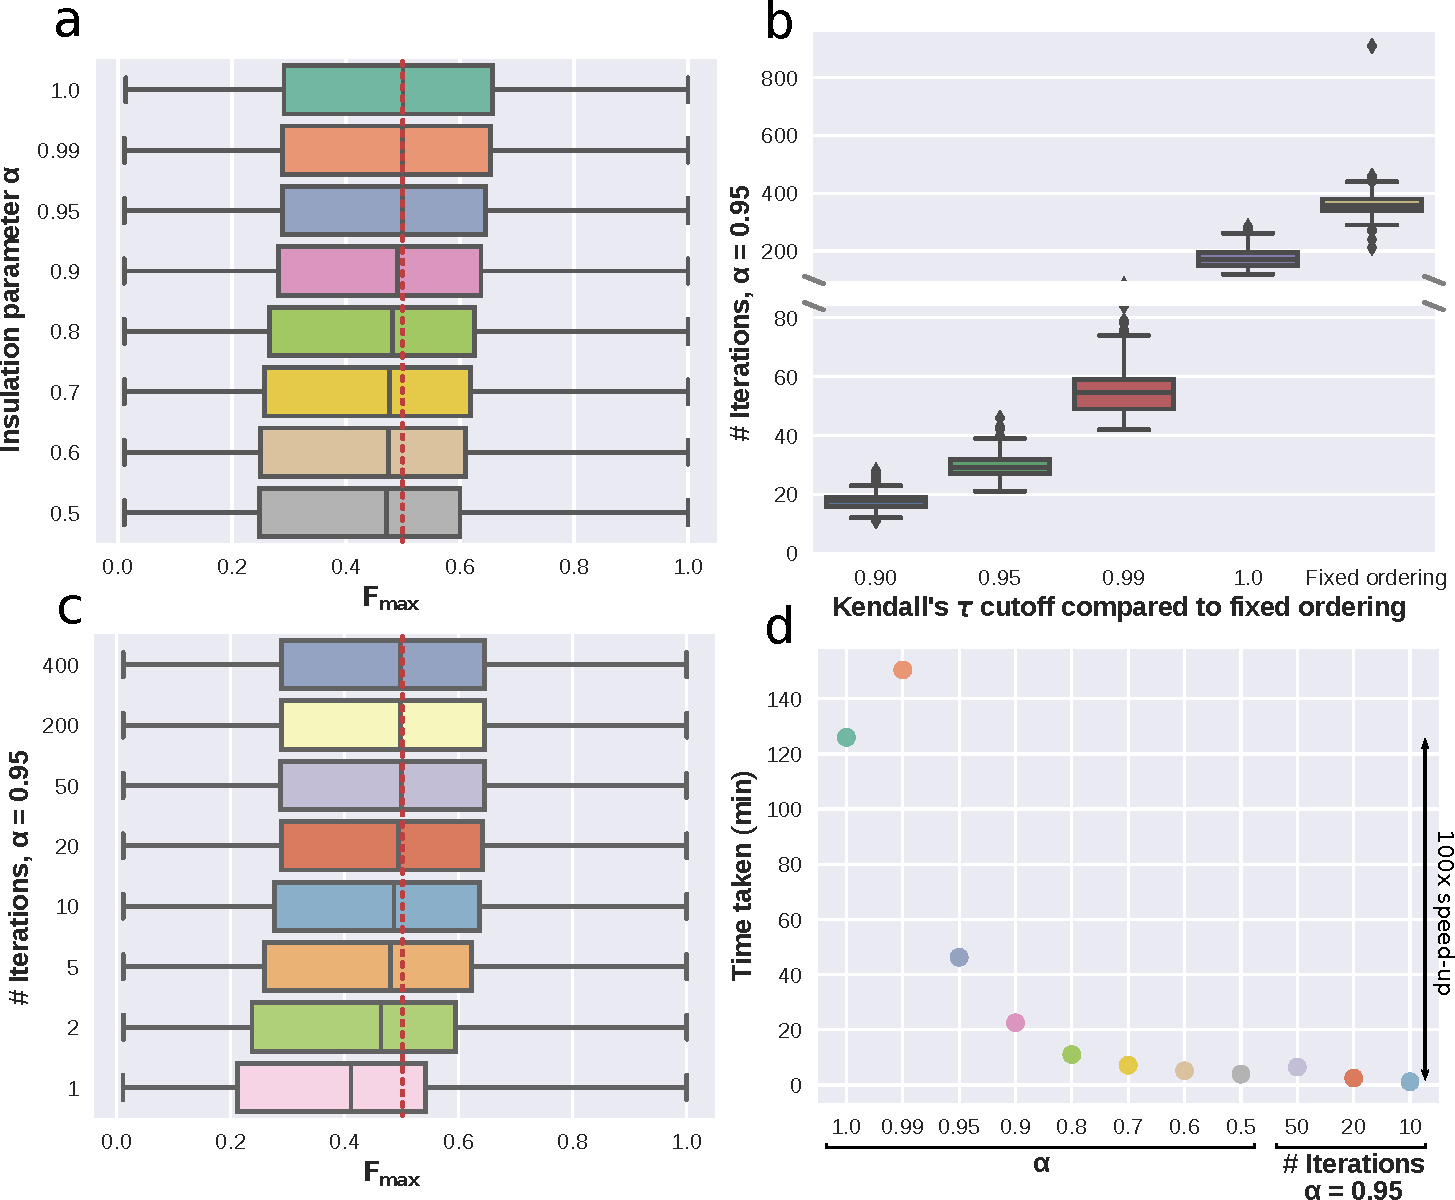
\includegraphics[width=\textwidth]{figs/fig1-2018_06-seq-sim-e0_1-string-expc-rem-neg-comp-iea-50-1000-bp-a0_95.pdf}
    \caption{Trade-off between accuracy and speed for \sinksource on the 19 bacterial species \SSN (\eval <= 0.1) with 319 BP GO terms ($\ge 50$ annotations) for the \loso evaluation. 
      %Performance is measured by computing the \fmax on a GO term by GO term basis. Here we used annotations of BP GO terms with experimental evidence codes
      (\textbf{a}) Variation of \fmax distributions with $\alpha$. The vertical red dotted line represents the median \fmax for $\alpha = 1.0$.
      (\textbf{b}) Number of iterations required to fix the rankings of the left-out positives and negatives, or to reach a specified value of \ktau in comparison to the fixed ranking.
      (\textbf{c}) Variation of \fmax distributions with the number of iterations ($\alpha=0.95$). The vertical red dotted line represents the median \fmax for $\alpha = 1.0$ in panel (a).
      (\textbf{d}) Total time taken by \sinksource (shown in a and b) while varying $\alpha$ or the number of iterations with $\alpha=0.95$. Colors are the same as in (\textbf{a}) and (\textbf{c}).
    }
    \label{fig:sinksource-speed-vs-accuracy}
\end{figure}

\subsection{Effect of BLAST \eval Cutoffs}
\label{sec:effect-eval-cutoffs}


Here, we studied the effect of using different \eval cutoffs to construct the sequence-similarity network, as this parameter can drastically change the size of the network (see Table \ref{tab:net-sizes}), with the largest \SSN containing over five million edges. 
%relatively high \evals can lead to spurious prediction results \jeff{TODO find citation}.
 

% evidence codes
In these evaluations, we first used annotations with at least one experimental evidence code. 
%for both making predictions, and evaluating the predictions.
%which is the standard set in CAFA~\cite{jiang-radivojac-cafa2-eval-function-prediction-gb-2016}.
As only a few species had a substantial number of experimentally-based annotations, we also expanded our evaluation to include annotations with either an experimental or computational evidence code, as well as all annotations regardless of evidence code (see \cref{sec:loso-results-expc-comp-iea}).

% BLAST cutoff makes a big difference for BP and MF
% network propagation still helps


When working with large networks, an initial approach may be to limit the number of edges using a stringent cutoff, and allow the propagation methods to make predictions using the edges with relatively high homology. 
%Such an approach is common when using a co-expression network \jeff{cite}.
Additionally, intuition would suggest that including many edges with relatively low homology would lead to more false positives \jeff{PFP and PhyloPFP used \evals up to 100. The BLAST webpage suggests a cutoff of \e{-6}, Effusion uses a cutoff of \e{-8}}. 

We tested cutoffs of \e{-25}, \e{-15}, \e{-6}, $0.1$, 5, 20 and 50 to evaluate at which cutoff we achieve the best performance.
We found that when we raised the \eval cutoff from \e{-25} to $0.1$, the median \fmax for each method increased by more than $0.1$ (rank-sum test \pval $4.2\times{}10^{-8}$, see \cref{fig:loso-results-exp}a,b).
Further raising the \eval cutoff past $0.1$ did not improve the median \fmax further (see Supplementary Text for results for \eval cutoffs of \e{-15} and \e{-6}, 5, 20, and 50).
We also observe that network propagation methods gain more of an advantage over \localplus for the more stringent \e{-25} cutoff than the 0.1 cutoff as expected, however we still see a marginal improvement at the 0.1 cutoff (rank-sum \pval = $3.5\times{}10^{-5}$ and $0.055$ respectively).

\begin{figure}[H]
    \centering
    %\jeff{figure placeholder}
    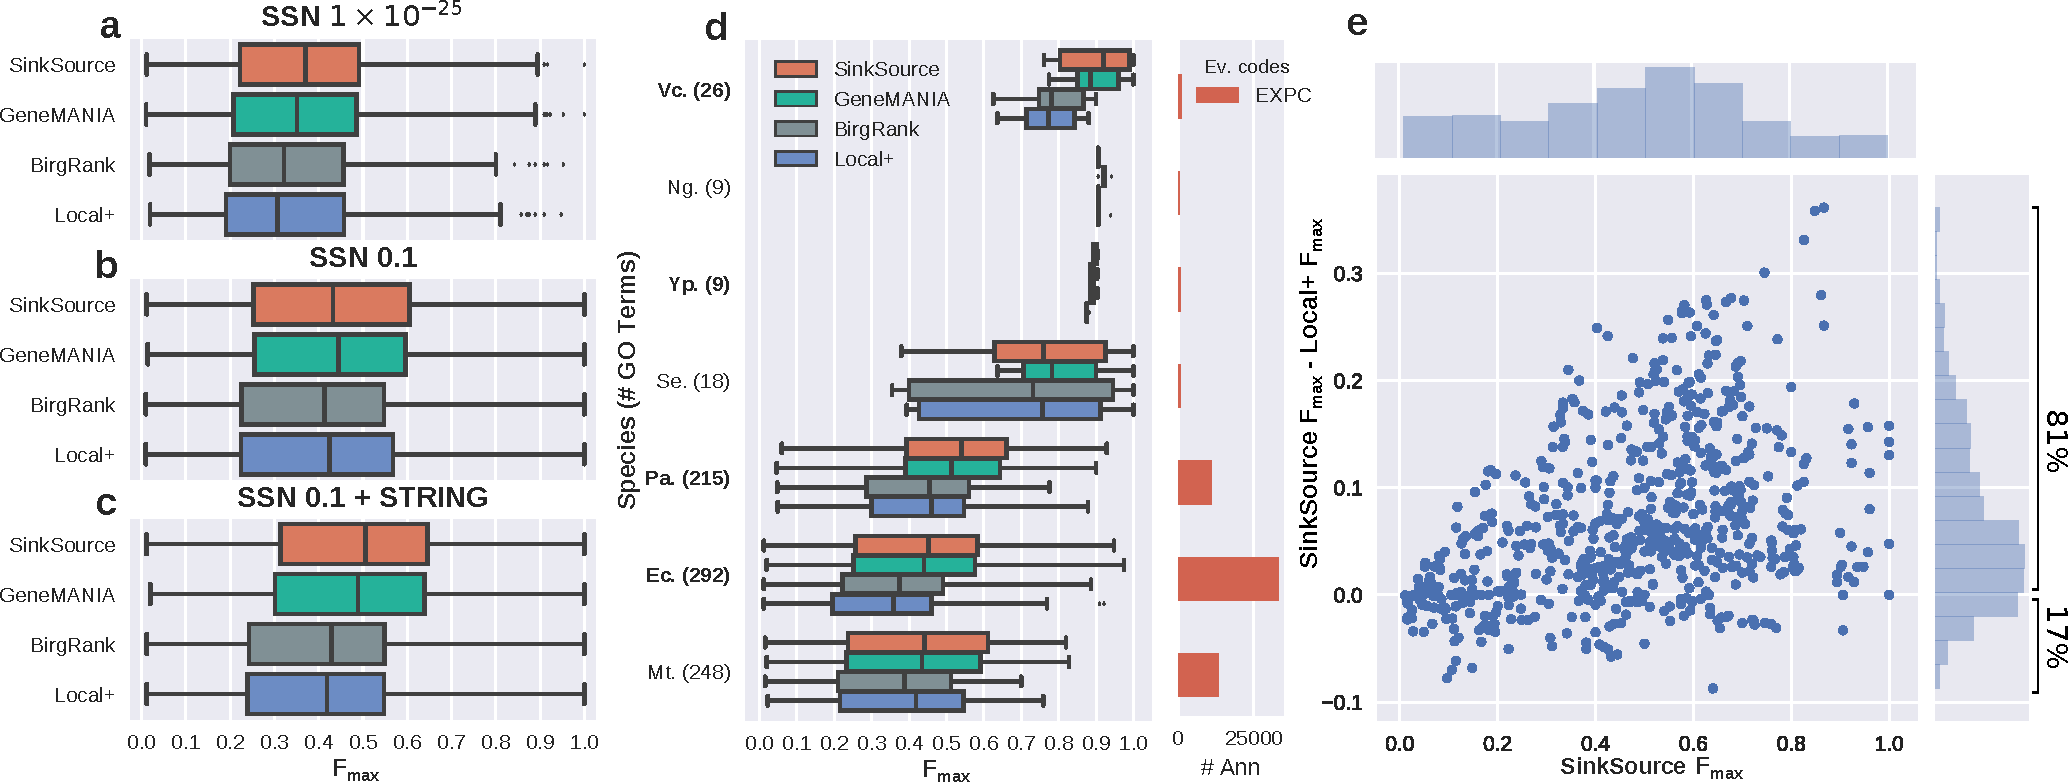
\includegraphics[width=\textwidth]{figs/fig2-expc-compare-eval-fmax-sinksource-localplus-bp-a0_95.pdf}
    \caption{
      Comparison of \fmax results for \loso evaluation across four algorithms and three networks.
      (\textbf{a}) \SSN (\eval $\le$ \e{-25}),
      (\textbf{b}) \SSN (\eval $\le$ 0.1),
      (\textbf{c},\textbf{d},\textbf{e}) \SSN (\eval $\le$ 0.1) integrated with STRING,
      (\textbf{d}) \loso results for individual species, sorted in decreasing order of median \fmax. The number of BP GO terms with $\ge$ 10 annotations appears in parentheses next to each species name.  The species name is in bold if the difference between the distributions for \sinksource and \localplus was statistically significant (rank-sum Bonferroni-corrected \pval $< 0.05$). \protect The right-hand side shows the number of GO term-annotation pairs with experimental evidence codes for each species.
    %315 total BP GO terms have at least 10 annotations in the left-out species. 
    Species names are abbreviated as follows:
    \textit{Escherichia coli K-12} (Ec),
    \textit{Mycobacterium tuberculosis} (Mt),
    \textit{Neisseria gonorrhoeae} (Ng),
    \textit{Pseudomonas aeruginosa} (Pa),
    \textit{Salmonella enterica} (Se),
    \textit{Vibrio cholerae} (Vc),
    \textit{Yersinia pestis} (Yp).
    (\textbf{e}) Difference in \fmax between \sinksource and \localplus by the \fmax of \sinksource for each GO term. 
    %Comparison of using a \SSN with a cutoff of $1\times{}10^{-25}$ vs. a cutoff of $0.1$. The \fmax results for each individual species are combined and shown in a single box-plot for each algorithm.}
    }
    \label{fig:loso-results-exp}
\end{figure}


\subsection{Incorporating STRING Networks}
\label{sec:loso-incorporate-string}
%Techniques which utilize multiple complementary data sources have been shown to be more accurate than those that use a single data source~\cite{jiang-radivojac-cafa2-eval-function-prediction-gb-2016, cozzetto-jones-pfp-massive-integration-bmcbioinfo-2013, gligorijevic-bonneau-deepnf-bioinfo-2018}.
%The STRING database is a great resource for multiple types of data (such as co-expression, protein-protein interactions)  available for many species \jeff{cite STRING}. A total of 14 out of 19 of our bacterial species have a matching strain in STRING. 
%We utilized six of the networks available in STRING (neighborhood, fusion, cooccurence, coexpression, experiments, and database).
We also integrated the STRING network for each bacterium into the sequence-similarity network. We sought to determine whether the integrated network yielded more accurate predictions than the sequence-similarity network itself. \murali{Give a reason for why integration is not just taking the union. And then what integration actually means here.} We tested two methods to perform this integration: \genemania-2008 and SWSN (see \cref{sec:network-integration}). 

% discussion section?
In our experiments we found that using the original integration method proposed by Mostafavi and Morris resulted in better performance than SWSN for \sinksource and \genemania, especially for MF GO terms (results not shown). \murali{Let us discuss the possibility of showing these results to the supplement. How different were the results?}
We used only the SWSN method for \birgrank as it requires a single network to make predictions for all GO terms simultaneously for each protein.

%First, the original method proposed by Mostafavi and Morris in 2008 where individual networks are given a score based on how well they agree with the positives and negatives of a given GO term, and then combined into a single network.
%Ultimately we found the original method proposed by Mostafavi and Morris in 2008 where individual networks are given a score based on how well they agree with the positives and negatives of a given GO term, and then combined into a single network, performed the best \cite{mostafavi-morris-genemania-gb-2008}.

We compared the effect of varying the cutoff for the quality of associations in the STRING networks.
\jeff{Need to discuss the different methods we tested for incorporating the STRING networks}.
%cutoffs as this can drastically change the size of the network (see Table \ref{tab:net-sizes}), with the largest network containing over 7.8M edges.
%Interestingly, we do not observe the same trend for STRING networks as we do for the \eval. \murali{What trend are you referring to for \eval? I think you can just delete the previous sentence.} 
We evaluated low, medium and high stringency cutoffs (150, 400 and 700 respectively) of the edge weights with the \SSN (\eval $\leq$ 0.1) using the same \loso approach. We used the cutoff of 400 for the remaining analyses since it gave a slight improvement of median \fmax over a cutoff of 150 and 700 (see the supplementary material). 

Comparing \cref{fig:loso-results-exp}b to \cref{fig:loso-results-exp}c, we observed that 
incorporating the STRING networks into the \SSN did not improve the results for \localplus, presumably because the the new intra-species edges were to other unknown examples in the left-out species. On the other hand, \sinksource and \genemania were able to utilize the additional information to improve predictions, increasing the median \fmax by about 0.05 for BP over using the \SSN only (\cref{fig:loso-results-exp}b vs \cref{fig:loso-results-exp}c) \jeff{Add the comparison to \localplus as well as the \pval}. The inclusion of STRING networks slightly decreased the performance for MF terms suggesting that the data in STRING was not useful for predicting these annotations (see \cref{fig:loso-results-exp-mf}. 

Table \ref{tab:loso-runtimes} contains the running times for each of the algorithms for the entire \loso evaluation. \sinksource was the fastest of the propagation methods. \murali{Looks out of place. Is there a better location? In any case, is there any salient point you want to mention here?}


\subsection{Species-specific results}
\label{sec:loso-species-specific}
We next considered the results for individual species of the \SSN (\eval $<$ 0.1) + STRING. We focused on seven (out of 19) organisms that had at least one BP GO term with at least 10 or more annotations in each species.
For four out of seven species, the improvement of \sinksource over \localplus was statistically significant (rank-sum Bonferroni-corrected \pval $< 0.05$, bold species abbreviations in \cref{fig:loso-results-exp}d). 
\genemania and \sinksource had very similar performance. 

We also noted considerable variation among species, with the median \fmax for \sinksource ranging from 0.41 to 0.92. The median \fmax for a species was negatively correlated with the number of annotations with experimental evidence codes for that organisms (right side of \cref{fig:loso-results-exp}d). 

% Mt doesn't really buck this trend, so I (Murali) am commenting out this paragraph.
%However, \textit{M. tuberculosis} does not seem to follow suit. \murali{It seems to follow this trend: between Pa and Ec for both median \fmax and \#annotations.} One hypothesis is that it is simply not as closely related to the other species, and is therefore more difficult to recover its annotations compared to the other species. Upon closer inspection of the phylogenetic tree of these 19 species, we see that \textit{M. tuberculosis} is the most distant, being the only species from the \textit{Actinobacteria} phylum (\jeff{see supp.}).

% wide spread
%\jeff{This doesn't quite fit here. The next section has more detail, but I want to include this in the discussion of A-D.}
We note there is a wide spread of prediction quality ranging from an \fmax of 0 to 1 across all GO terms. 
This is likely due to the fact that we consider GO terms with a wide range of specificities, causing our \fmax values to also span a wide range. 
For many GO terms, a large percentage of annotations are for a single species \jeff{need some statistics for that.}, making the problem either more difficult for that species if it is left-out, or relatively easy when other species are left-out. 
However, the main point we seek to address is whether or not there is a systematic GO term by GO term difference between \sinksource and \localplus which is what we investigated next. %observe in \fig \ref{fig:loso-results-exp}e (described below).


\subsection{Improvement of \sinksource over \localplus}  
\label{sec:loso-sinksource-localplus}
We sought to examine in more depth how often, and why the network propagation methods \sinksource and \genemania are gaining an advantage over \localplus.
Directly comparing the \fmax values of \sinksource and \localplus for each GO term individually, we see that for over 75\% of them, network propagation offers an improvement in prediction performance over only considering immediate neighbors (see \cref{fig:loso-results-exp}e), while \localplus does slightly better than \sinksource for 14\% of GO terms.
\jeff{What about for MF? \genemania?}

We also observe a trend that as the \fmax values for \localplus increase, the improvement of \sinksource over \localplus increases also increases. 
This suggests that as the number of positives in the 18 species that are close to the left-out positives increases, network propagation is better able to utilize the additional information.
But when there are little to no positives nearby (low \localplus \fmax), \sinksource also does poorly.
%This seems to suggest that network propagation methods are better able to distinguish positive examples from negative examples by utilizing multiple short paths around the positives.  

Looking more into why network propagation does better, we examined the distance of the left-out positives to the positives in the network.  
We found that in the cases where network propagation does better, there are multiple short paths (length 2-3) to the positives, distinguishing left-out positives from other proteins (left-out negatives). 
\jeff{Figure showing for an example GO term (or many GO terms) the distances of left-out positives to training positives?}
Figure \ref{fig:sos-response-sinksource-vs-localplus} shows a simple example where for 5 out of 15 \textit{P. aeruginosa} proteins annotated to the GO term ``SOS response'' (GO:0009432), there is no direct connection to a positive causing them to be missed by \localplus, yet \sinksource is able to rank them highly~\jeff{Need to include the fifth node}.
\jeff{I want to include the unknowns which are also ranked highly. Many of them have COMP or ELEC annotations to SOS response or a closely related GO term DNA damage response.}
We chose this GO term as an example as it has a large \fmax improvement (0.18) for \sinksource over \localplus (0.93 and 0.75 respectively), a relatively small number of annotations (making it easier to visualize) and it has been shown to be involved in resistance to antibiotics~\jeff{include description from paper(s)}.

Another benefit of network propagation is the fact that the ranks for \localplus stop at 43 as all nodes after 42 are tied with a score of 0, meaning they have no direct connections to a positive. 
\sinksource on the other hand is able to give scores for almost all of the 5,575 \textit{P. aeruginosa} proteins.
%This is a bit of a simple 

\begin{figure}[H]
    \centering
    %\jeff{need to fix figure headings}
    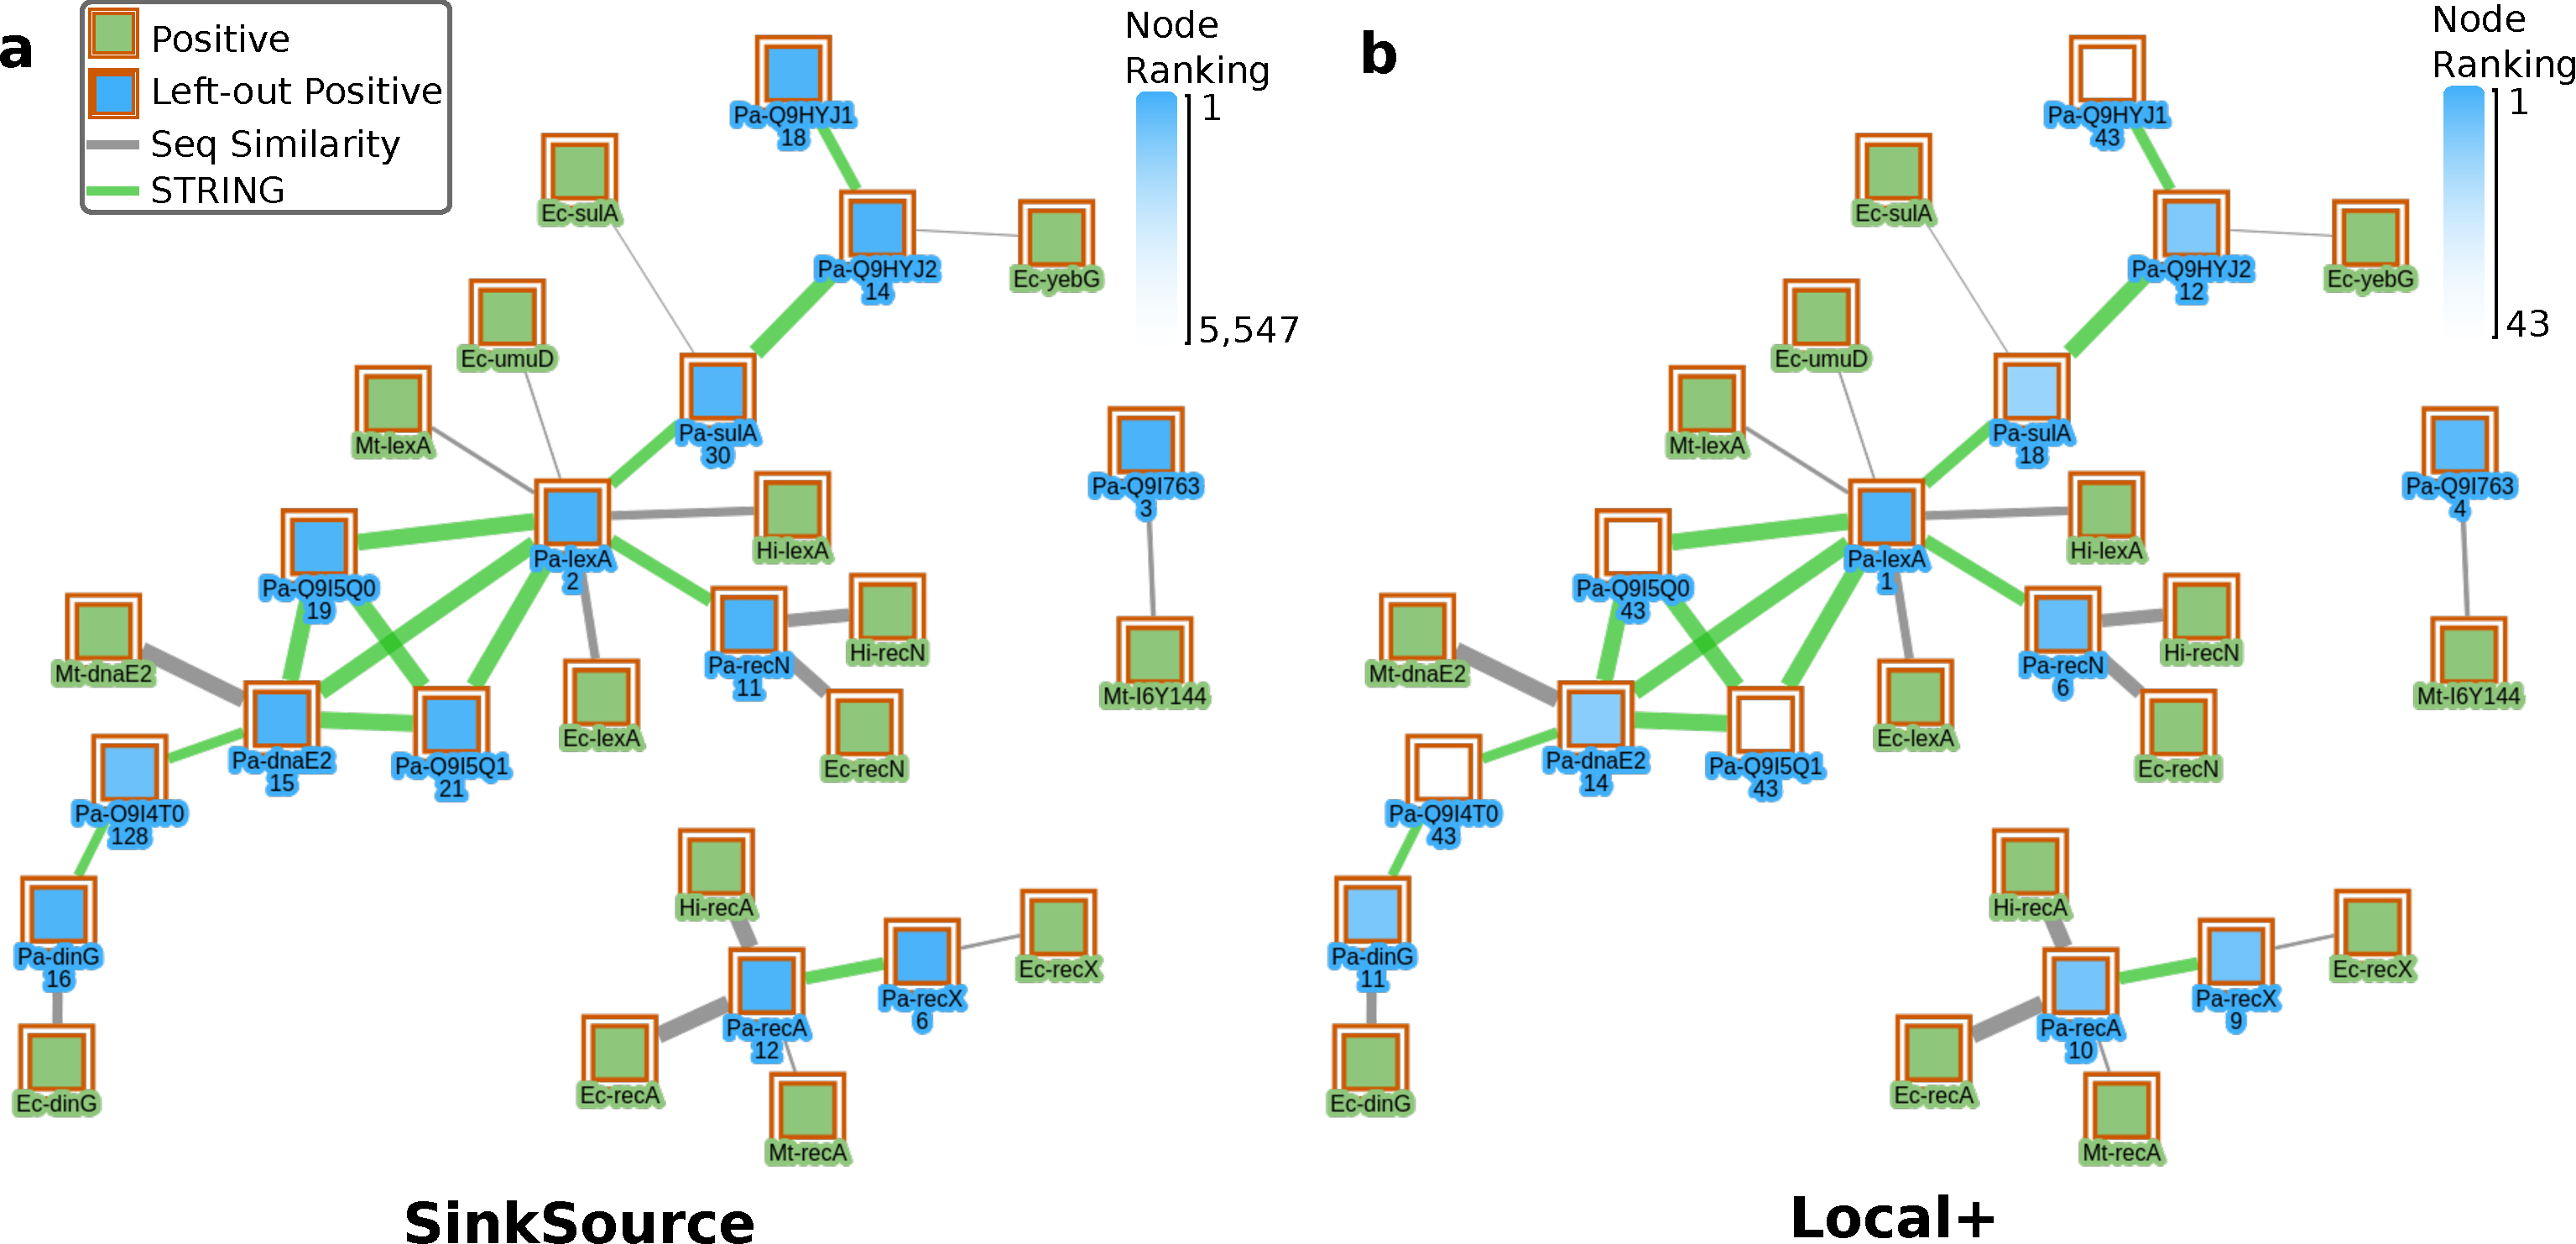
\includegraphics[width=\textwidth]{figs/fig4-sinksource-vs-localplus-sos-response.pdf}
    %\jeff{Add a scatterplot or something of the number of iterations and the median \fmax. Also add # of iterations and time taken}
    \caption{\sinksource comparison to \localplus. 
    Node rankings for left-out positives (blue) of \textit{P. aeruginosa} for example GO term "SOS response" GO:0009432. Nodes are colored by their rank.
    (a) \sinksource, (b) \localplus. \localplus is only able to give scores to 43 nodes, while \sinksource gives scores to almost all of the 5,575 \textit{P. aeruginosa} proteins.
    Species abbrev. same as in the caption of \cref{fig:loso-results-exp}.
    }
    \label{fig:sos-response-sinksource-vs-localplus}
\end{figure}


\begin{table}[htb]
    \centering
    \begin{tabular}{l|r|l}
    Method & Total Time (min) & Solver \\
    \hline
    \sinksource & 2.6  & 10 Iterations, $\alpha=0.95$ \\
    \genemania  & 44.0 & Conjugate Gradient ($tol=\e{-5}$) \\
    \birgrank   & 19.5 & Power Iteration ($\epsilon=\e{4}$) \\
    \localplus  & 0.3  & 1 Iteration \\
    \end{tabular}
    \caption{Total processor time of the four methods in minutes (\loso, BP terms, EXPC annotations) along with the type of solver used for each method. For \genemania, the reported time is the total process time used by CG across eight cores.}
    %\jeff{TODO times of weighting methods. SWSN: 6.4 min, indv GO terms 14.4 min (SS and \localplus), GM indv 39.9 min}
    \label{tab:loso-runtimes}
\end{table}


% EXPC + COMP, evaluate COMP
% EXPC + COMP + IEA, evaluate IEA
\subsection{LOSO Evaluation with Computational and Electronic Evidence Codes}
\label{sec:loso-results-expc-comp-iea}

\begin{figure}[H]
    \centering
    %\jeff{need to fix figure headings}
    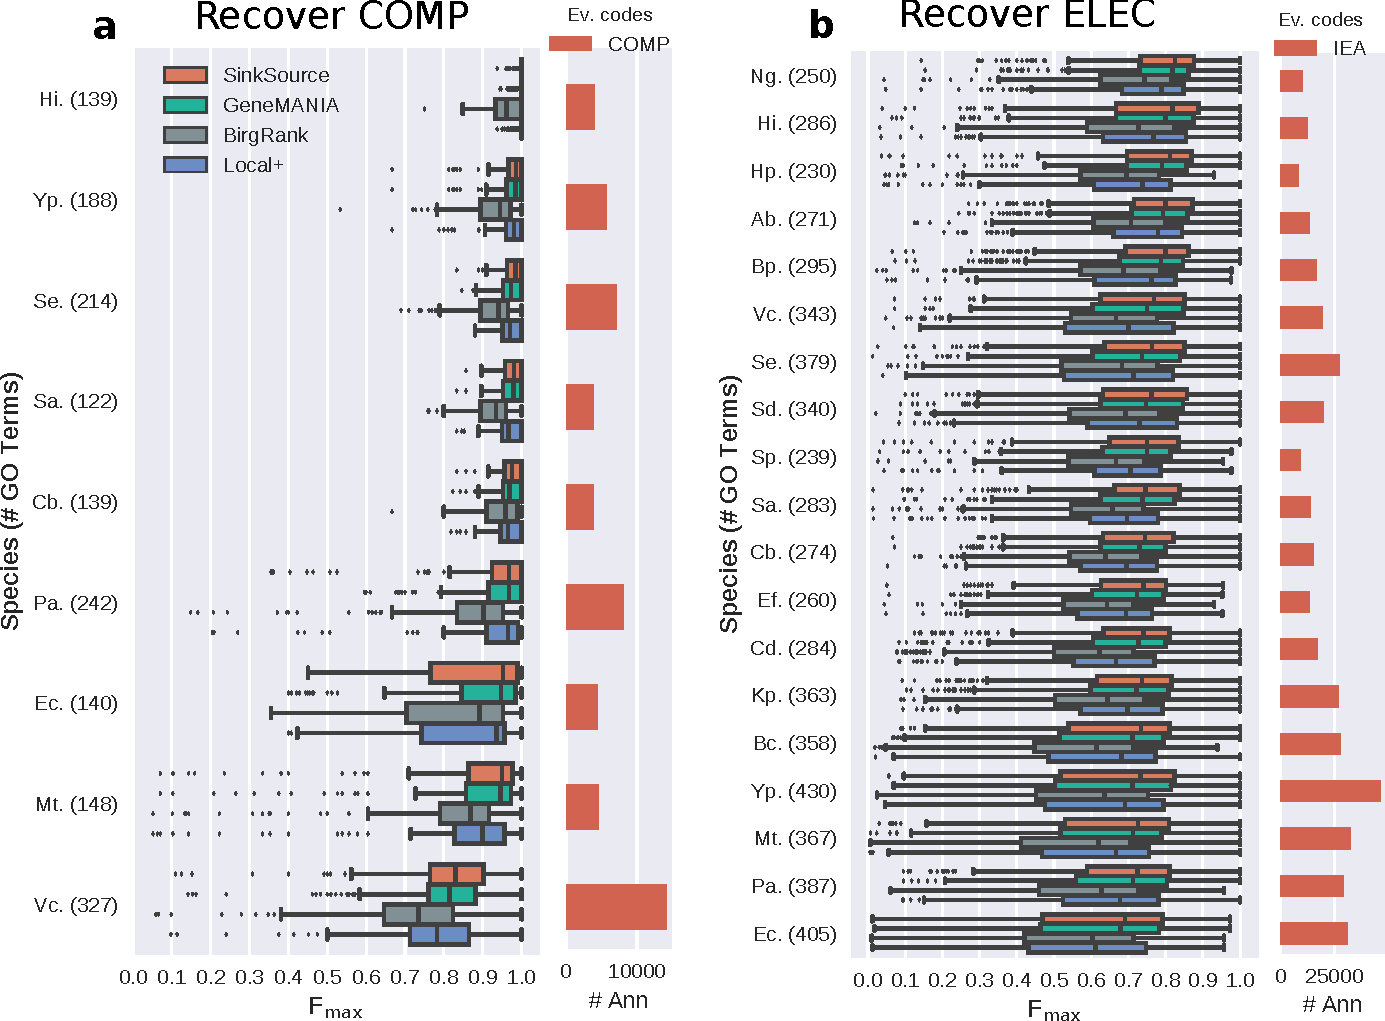
\includegraphics[width=\textwidth]{figs/fig3-expc-comp-iea.pdf}
    %\jeff{Add a scatterplot or something of the number of iterations and the median \fmax. Also add # of iterations and time taken}
    \caption{
      Comparison of \fmax results for the \loso evaluation for different evidence codes using the \SSN (\eval $\le$ 0.1) integrated with STRING. We made predictions using annotations with EXP and COMP evidence codes.
      (\textbf{a}) Evaluation of recovery of COMP evidence codes of the left-out species.
      (\textbf{b}) Evaluation of recovery of ELEC evidence codes (IEA) of the left-out species.
      Additional species names not defined in \cref{fig:loso-results-exp} are abbreviated as follows:
      \textit{Acinetobacter baumannii} (Ab), 
      \textit{Burkholderia cepacia} (Bc), 
      \textit{Bordetella pertussis} (Bp), 
      \textit{Clostridium botulinum} (Cb),
      \textit{Clostridioides difficile} (Cd), 
      \textit{Enterococcus faecium} (Ef),
      \textit{Haemophilus influenzae} (Hi),
      \textit{Helicobacter pylori} (Hp), 
      \textit{Klebsiella pneumoniae} (Kp),
      \textit{Staphylococcus aureus} (Sa),
      \textit{Shigella dysenteriae} (Sd),
      \textit{Streptococcus pyogenes} (Sp)
    }
    \label{fig:loso-results-expc-comp-iea}
\end{figure}

As most of our 19 organisms had little to no annotations based on experimental evidence (EXP), we expanded our analysis to include more organisms by mimicking the experimentally-based annotations with annotations based on computational analysis (COMP). 
%We evaluated and compare our methods using annotations with computational analysis evidence codes which are manually performed by a curator using sequence similarity (COMP), as well as automatic annotations with electronic evidence codes (ELEC). 
We repeated our \loso analysis using EXP and COMP annotations in 18 species, and evaluated each method's ability to recover the COMP annotations in the left-out species. A total of nine organisms had at least one BP GO term with 10 or more COMP annotations.

As expected, we immediately observed that recovering COMP annotations using a \SSN is much easier than recovering EXP annotations (see \cref{fig:loso-results-expc-comp-iea}a. For X/9 species, the improvement over \localplus was statistically significant.  

%\subsection{Temporal Holdout Evaluation}
%June 2016 - September 2017

\subsection{Scaling to 200 Bacterial Species}
\label{sec:loso-s200}

To test the ability of our methods to scale to include many more species, we built a \SSN with 200 bacterial species. 
%These species were chosen based on the criteria 
We chose the top 200 bacterial species with the most GO annotations with experimental and computational evidence codes. 
These species had a wide range of genome sizes varying from  protein-coding genes \jeff{TODO}. 
% 6,676 to 438 genes with at least one annotation (for \textit{Streptomyces bingchenggensis} NCBI:txid749414 and \textit{Mycoplasma genitalium} NCBI:txid243273 respectively) 
We also used an \eval cutoff of 0.1 for this \SSN, which yielded a network with 815K total proteins and 73M edges.
A total of 711 BP GO terms had 50 or more EXP or COMP annotations summed across the 200 species. 

We repeated the \loso evaluation with EXP and COMP annotations as in \cref{fig:loso-results-expc-comp-iea} with the 200 bacterial species where for each species in turn, we left-out all annotations for that species, then ran each algorithm with the EXP and COMP annotations to evaluate our ability to recover the left-out annotations. Rather than show the results for all 200 species individually, we summarized the results in \cref{tab:s200-loso-comp-iea}. 

We first observe the median \fmax of each algorithm are fairly similar to those in \cref{fig:loso-results-expc-comp-iea} and many of the observations made in that section remain true here. 
\jeff{Do the distributions for the 19-species increase?}
%Additionally, we find that 
% \jeff{Does the # of significant species increase? decrease? stay the same?}

\begin{table}[H]
    \centering
    \subfloat[Recover COMP]{
\begin{tabular}{|lccc|}
\hline 
Algorithm & Median  & MAD & \# Sig. Sp.\\
 & \fmax &  & (out of 42)\\
\hline
SinkSource & 0.984 & 0.02 & -\\
GeneMANIA & 0.984 & 0.02 & 0\\
BirgRank & 0.957 & 0.04 & 33\\
Local+ & 0.976 & 0.02 & 6\\
\hline 
\end{tabular}
    }
\quad
    \subfloat[Recover ELEC]{
\begin{tabular}{|lccc|}
\hline 
Algorithm & Median & MAD  & \# Sig. Sp.\\
 & \fmax  &  & (out of 200)\\
\hline
SinkSource & 0.750 & 0.09 & -\\
GeneMANIA & 0.756 & 0.10 & 0\\
BirgRank & 0.600 & 0.13 & 188\\
Local+ & 0.711 & 0.10 & 51\\
% with 20 iterations, 88 species are significant
\hline 
\end{tabular}
}

    \caption{
      Comparison of \fmax results of the \loso evaluation of different evidence codes using EXP and COMP annotations to make predictions for 200 bacterial species. MAD stands for Median Absolute Deviation. The column titled "\# Sig. Sp." shows the number of species for which the \fmax improvement of \sinksource over the given algorithm was statistically significant (rank-sum test, corrected by number of species)
      (\textbf{a}) Evaluation of recovery of COMP evidence codes of the left-out species. Total number of species - GO term pairs: 6,951.
      (\textbf{b}) Evaluation of recovery of ELEC evidence codes (IEA) of the left-out species. Total number of species - GO term pairs: 73,708.
}
    \label{tab:s200-loso-comp-iea}
\end{table}


% TODO include the total time in the previous table?
% \begin{table}[]
%     \centering
%     \begin{tabular}{c|c}
%          &  \\
%          & 
%     \end{tabular}
%     \caption{Total processor time of the four methods in hours}
%     \label{tab:my_label}
% \end{table}